\PassOptionsToPackage{unicode=true}{hyperref} % options for packages loaded elsewhere
\PassOptionsToPackage{hyphens}{url}
%
\documentclass[ignorenonframetext,aspectratio=169]{beamer}
\usepackage{pgfpages}
\setbeamertemplate{caption}[numbered]
\setbeamertemplate{caption label separator}{: }
\setbeamercolor{caption name}{fg=normal text.fg}
\beamertemplatenavigationsymbolsempty
% Prevent slide breaks in the middle of a paragraph:
\widowpenalties 1 10000
\raggedbottom
\setbeamertemplate{part page}{
\centering
\begin{beamercolorbox}[sep=16pt,center]{part title}
  \usebeamerfont{part title}\insertpart\par
\end{beamercolorbox}
}
\setbeamertemplate{section page}{
\centering
\begin{beamercolorbox}[sep=12pt,center]{part title}
  \usebeamerfont{section title}\insertsection\par
\end{beamercolorbox}
}
\setbeamertemplate{subsection page}{
\centering
\begin{beamercolorbox}[sep=8pt,center]{part title}
  \usebeamerfont{subsection title}\insertsubsection\par
\end{beamercolorbox}
}
\AtBeginPart{
  \frame{\partpage}
}
\AtBeginSection{
  \ifbibliography
  \else
    \frame{\sectionpage}
  \fi
}
\AtBeginSubsection{
  \frame{\subsectionpage}
}
\usepackage{lmodern}
\usepackage{amssymb,amsmath}
\usepackage{ifxetex,ifluatex}
\usepackage{fixltx2e} % provides \textsubscript
\ifnum 0\ifxetex 1\fi\ifluatex 1\fi=0 % if pdftex
  \usepackage[T1]{fontenc}
  \usepackage[utf8]{inputenc}
  \usepackage{textcomp} % provides euro and other symbols
\else % if luatex or xelatex
  \usepackage{unicode-math}
  \defaultfontfeatures{Ligatures=TeX,Scale=MatchLowercase}
\fi
\usetheme[]{Frankfurt}
\usecolortheme{beaver}
% use upquote if available, for straight quotes in verbatim environments
\IfFileExists{upquote.sty}{\usepackage{upquote}}{}
% use microtype if available
\IfFileExists{microtype.sty}{%
\usepackage[]{microtype}
\UseMicrotypeSet[protrusion]{basicmath} % disable protrusion for tt fonts
}{}
\IfFileExists{parskip.sty}{%
\usepackage{parskip}
}{% else
\setlength{\parindent}{0pt}
\setlength{\parskip}{6pt plus 2pt minus 1pt}
}
\usepackage{hyperref}
\hypersetup{
            pdftitle={Conservation of biodiversity -- current practices national legislation and international conventions and treaties, and biodiversity prospects and intellectual property rights.},
            pdfauthor={Deependra Dhakal},
            pdfborder={0 0 0},
            breaklinks=true}
\urlstyle{same}  % don't use monospace font for urls
\newif\ifbibliography
\setlength{\emergencystretch}{3em}  % prevent overfull lines
\providecommand{\tightlist}{%
  \setlength{\itemsep}{0pt}\setlength{\parskip}{0pt}}
\setcounter{secnumdepth}{0}

% set default figure placement to htbp
\makeatletter
\def\fps@figure{htbp}
\makeatother

\usepackage{booktabs}
\usepackage{longtable}
\usepackage{array}
\usepackage{multirow}
\usepackage{wrapfig}
\usepackage{float}
\usepackage{colortbl}
\usepackage{pdflscape}
\usepackage{tabu}
\usepackage{threeparttable}
\usepackage{threeparttablex}
\usepackage[normalem]{ulem}
\usepackage{makecell}
\usepackage{xcolor}
\usepackage{tikz} % required for image opacity change
\usepackage[absolute,overlay]{textpos} % for text formatting

% this font option is amenable for beamer
\setbeamerfont{caption}{size=\tiny}

\title{Conservation of biodiversity -- current practices national legislation
and international conventions and treaties, and biodiversity prospects
and intellectual property rights.}
\author{Deependra Dhakal}
\providecommand{\institute}[1]{}
\institute{GAASC, Baitadi \and Tribhuwan University}
\date{Academic year 2019-2020}

\begin{document}
\frame{\titlepage}

\begin{frame}
\tableofcontents[hideallsubsections]
\end{frame}
\hypertarget{biodiversity-conservation}{%
\section{Biodiversity conservation}\label{biodiversity-conservation}}

\begin{frame}{Background}
\protect\hypertarget{background}{}

\begin{itemize}
\tightlist
\item
  Conservationists' focus has expanded from the objective of
  establishing beautiful parks and conserving select species towards a
  more holistic goal of ecosystem integrity; a goal that goes well
  beyond the conservation of individual species and beautiful landscapes
  to include the protection of the existing diversity of species,
  natural habitats, and ecosystem processes.
\item
  Fundamental questions about goals and strategies, particularly

  \begin{enumerate}
  \tightlist
  \item
    What biodiversity should be conserved; e.g., should the focus be
    particular species, ecosystems, or ecosystem services?
  \item
    Where does the targeted biodiversity occur, and where is the best
    place to protect it? and
  \item
    Given the variety of conservation tools available, which is the most
    effective method to achieve conservation objectives?
  \end{enumerate}
\item
  Traditional form of contribution to conservation effort due following
  peoples:

  \begin{itemize}
  \tightlist
  \item
    Geographers
  \item
    Ethnobotanists
  \item
    Plant ecologists
  \end{itemize}
\item
  Interplay of physical diversity and human management diversity gives
  rise complexity in agrobiodiversity.
\end{itemize}

\end{frame}

\begin{frame}{Operational considerations}
\protect\hypertarget{operational-considerations}{}

\begin{itemize}
\tightlist
\item
  Hotspots approach to defining what should be conserved or
  coarse-filter/fine-filter approach that ensures that a given
  landscape's naturally occuring species and ecological communities are
  protected.
\item
  Identifying the appropriate conservation landscape scale (Species/taxa
  or spatial scale)
\item
  Need for multiple conservation operational tools (Governance based,
  Market based, Civil society based)
\item
  Economic evaluation and conservation trade-offs with competing
  resource demands
\item
  Use of ``easy'' tools (i.e., GIS models and remote sensing data) to
  resolve ecological features and processes and design interventions.
\end{itemize}

\end{frame}

\hypertarget{causes-of-biodiversity-loss}{%
\section{Causes of biodiversity
loss}\label{causes-of-biodiversity-loss}}

\begin{frame}{Major drivers}
\protect\hypertarget{major-drivers}{}

\begin{itemize}
\tightlist
\item
  Habitat loss, overexploitation, alien species introductions, and
  climate change have resulted in significant losses to biodiversity,
  especially over the past 50 years.
\item
  These drivers are a influential both in protected as well as open
  areas.
\item
  Within protected areas

  \begin{itemize}
  \tightlist
  \item
    range of physical (e.g., fire),
  \item
    biological (e.g., alien species),
  \item
    social (e.g., community opposition),
  \item
    political (e.g., political support),
  \item
    economic (lack of resources), and
  \item
    managerial (e.g., lack of planning) threats are faced by
    biodiversity
  \end{itemize}
\end{itemize}

\end{frame}

\hypertarget{forms-of-biodiversity-conservation}{%
\section{Forms of biodiversity
conservation}\label{forms-of-biodiversity-conservation}}

\begin{frame}{On farm conservation}
\protect\hypertarget{on-farm-conservation}{}

\begin{itemize}
\tightlist
\item
  Seed preservation by farmer household
\item
  Participatory variety breeding
\item
  Culture based importance for conservation
\end{itemize}

\end{frame}

\begin{frame}{Protected area conservation: History}
\protect\hypertarget{protected-area-conservation-history}{}

\begin{itemize}
\tightlist
\item
  As long as 2000 years ago ancient societies in Greece, Rome, Asia, and
  Africa are known to have set aside areas as sacred groves or sites,
  while european societies had hunting grounds for use of royalty and
  the wealthy.
\item
  First protected area of world: Yellowstone National Park (1872).
\item
  Until recently, the motivations have seldom been the protection of
  biodiversity \emph{per se}, and have usually been based on culturally
  valued aspects of biodiversity and the broader landscape, for example,
  charismatic megafauna, attractive habitats, important watersheds,
  recreational areas, or endangered species.
\item
  Multiple functions of protected areas:

  \begin{itemize}
  \tightlist
  \item
    Scientific research,
  \item
    Wilderness protection,
  \item
    Preservation of species and genetic diversity,
  \item
    Maintenance of environmental services,
  \item
    Protection of specific natural and cultural features,
  \end{itemize}
\end{itemize}

\end{frame}

\begin{frame}{}
\protect\hypertarget{section}{}

\begin{itemize}
\tightlist
\item
  Multiple functions \ldots{}

  \begin{itemize}
  \tightlist
  \item
    Tourism and recreation,
  \item
    Education,
  \item
    Sustainable use of resources from natural ecosystems, and
  \item
    Maintenance of cultural and traditional attributes
  \end{itemize}
\end{itemize}

\end{frame}

\begin{frame}{Protected area: Components}
\protect\hypertarget{protected-area-components}{}

\begin{block}{International Union for Conservation of Nature}
A clearly defined geographical space, recognized, dedicated and managed through legal or other effective means, to achieve the long-term conservation of nature with associated ecosystem services and cultural values.
\end{block}

\begin{itemize}
\tightlist
\item
  12.9\% (114,000 sites) of earth's land surface now occur under
  protected areas.
\end{itemize}

\end{frame}

\begin{frame}{}
\protect\hypertarget{section-1}{}

\begin{itemize}
\tightlist
\item
  IUCN categories of protected areas: 1a. Strict Nature Reserves; Areas
  set aside to protect biodiversity and possibly geological features
  within strict control of visitation, use and impact. 1b. Wilderness
  Areas; Largely unmodified or slightly modified area, retaining natural
  character without human habitation.

  \begin{enumerate}
  \setcounter{enumi}{1}
  \tightlist
  \item
    National Parks; Natural or near natural areas to protect large scale
    ecological processes
  \item
    Natural Monuments or Features; Landform, Sea mount, Submarine
    cavern, Cave, Living creature
  \item
    Habitat/Species Management Areas; Particular species or habitats and
    management
  \item
    Protected Landscape/Seascape: Area of interaction of people and
    nature
  \item
    Protected area with sustainable use: Large area, low level
    industrial use of natural resource, with cultural associations for
    natural resource management.
  \end{enumerate}
\end{itemize}

\end{frame}

\begin{frame}{Status of protected areas}
\protect\hypertarget{status-of-protected-areas}{}

\begin{figure}
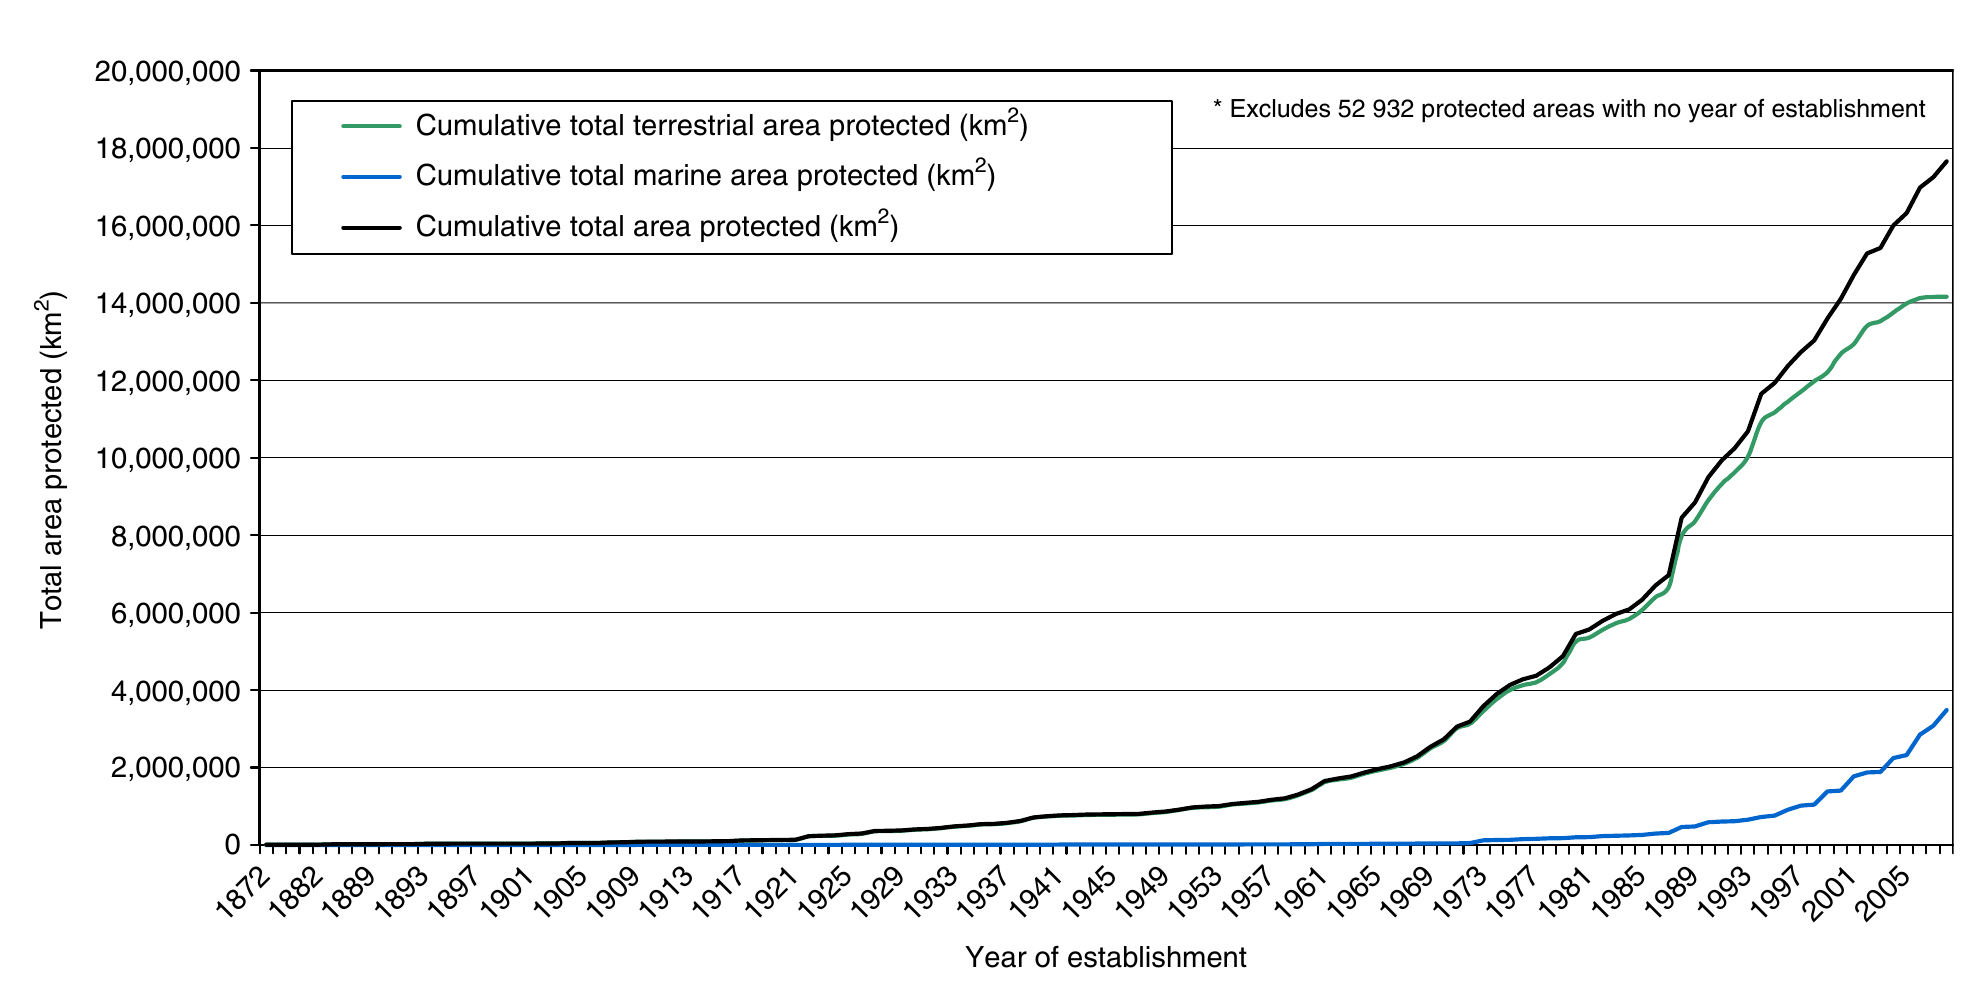
\includegraphics[width=0.65\linewidth]{./../images/global_protected_area} \caption{Global growth in protected areas. Reproduced from IUCN and UNEP-WCMC (2009).}\label{fig:global}
\end{figure}

\end{frame}

\begin{frame}{}
\protect\hypertarget{section-2}{}

\begin{figure}
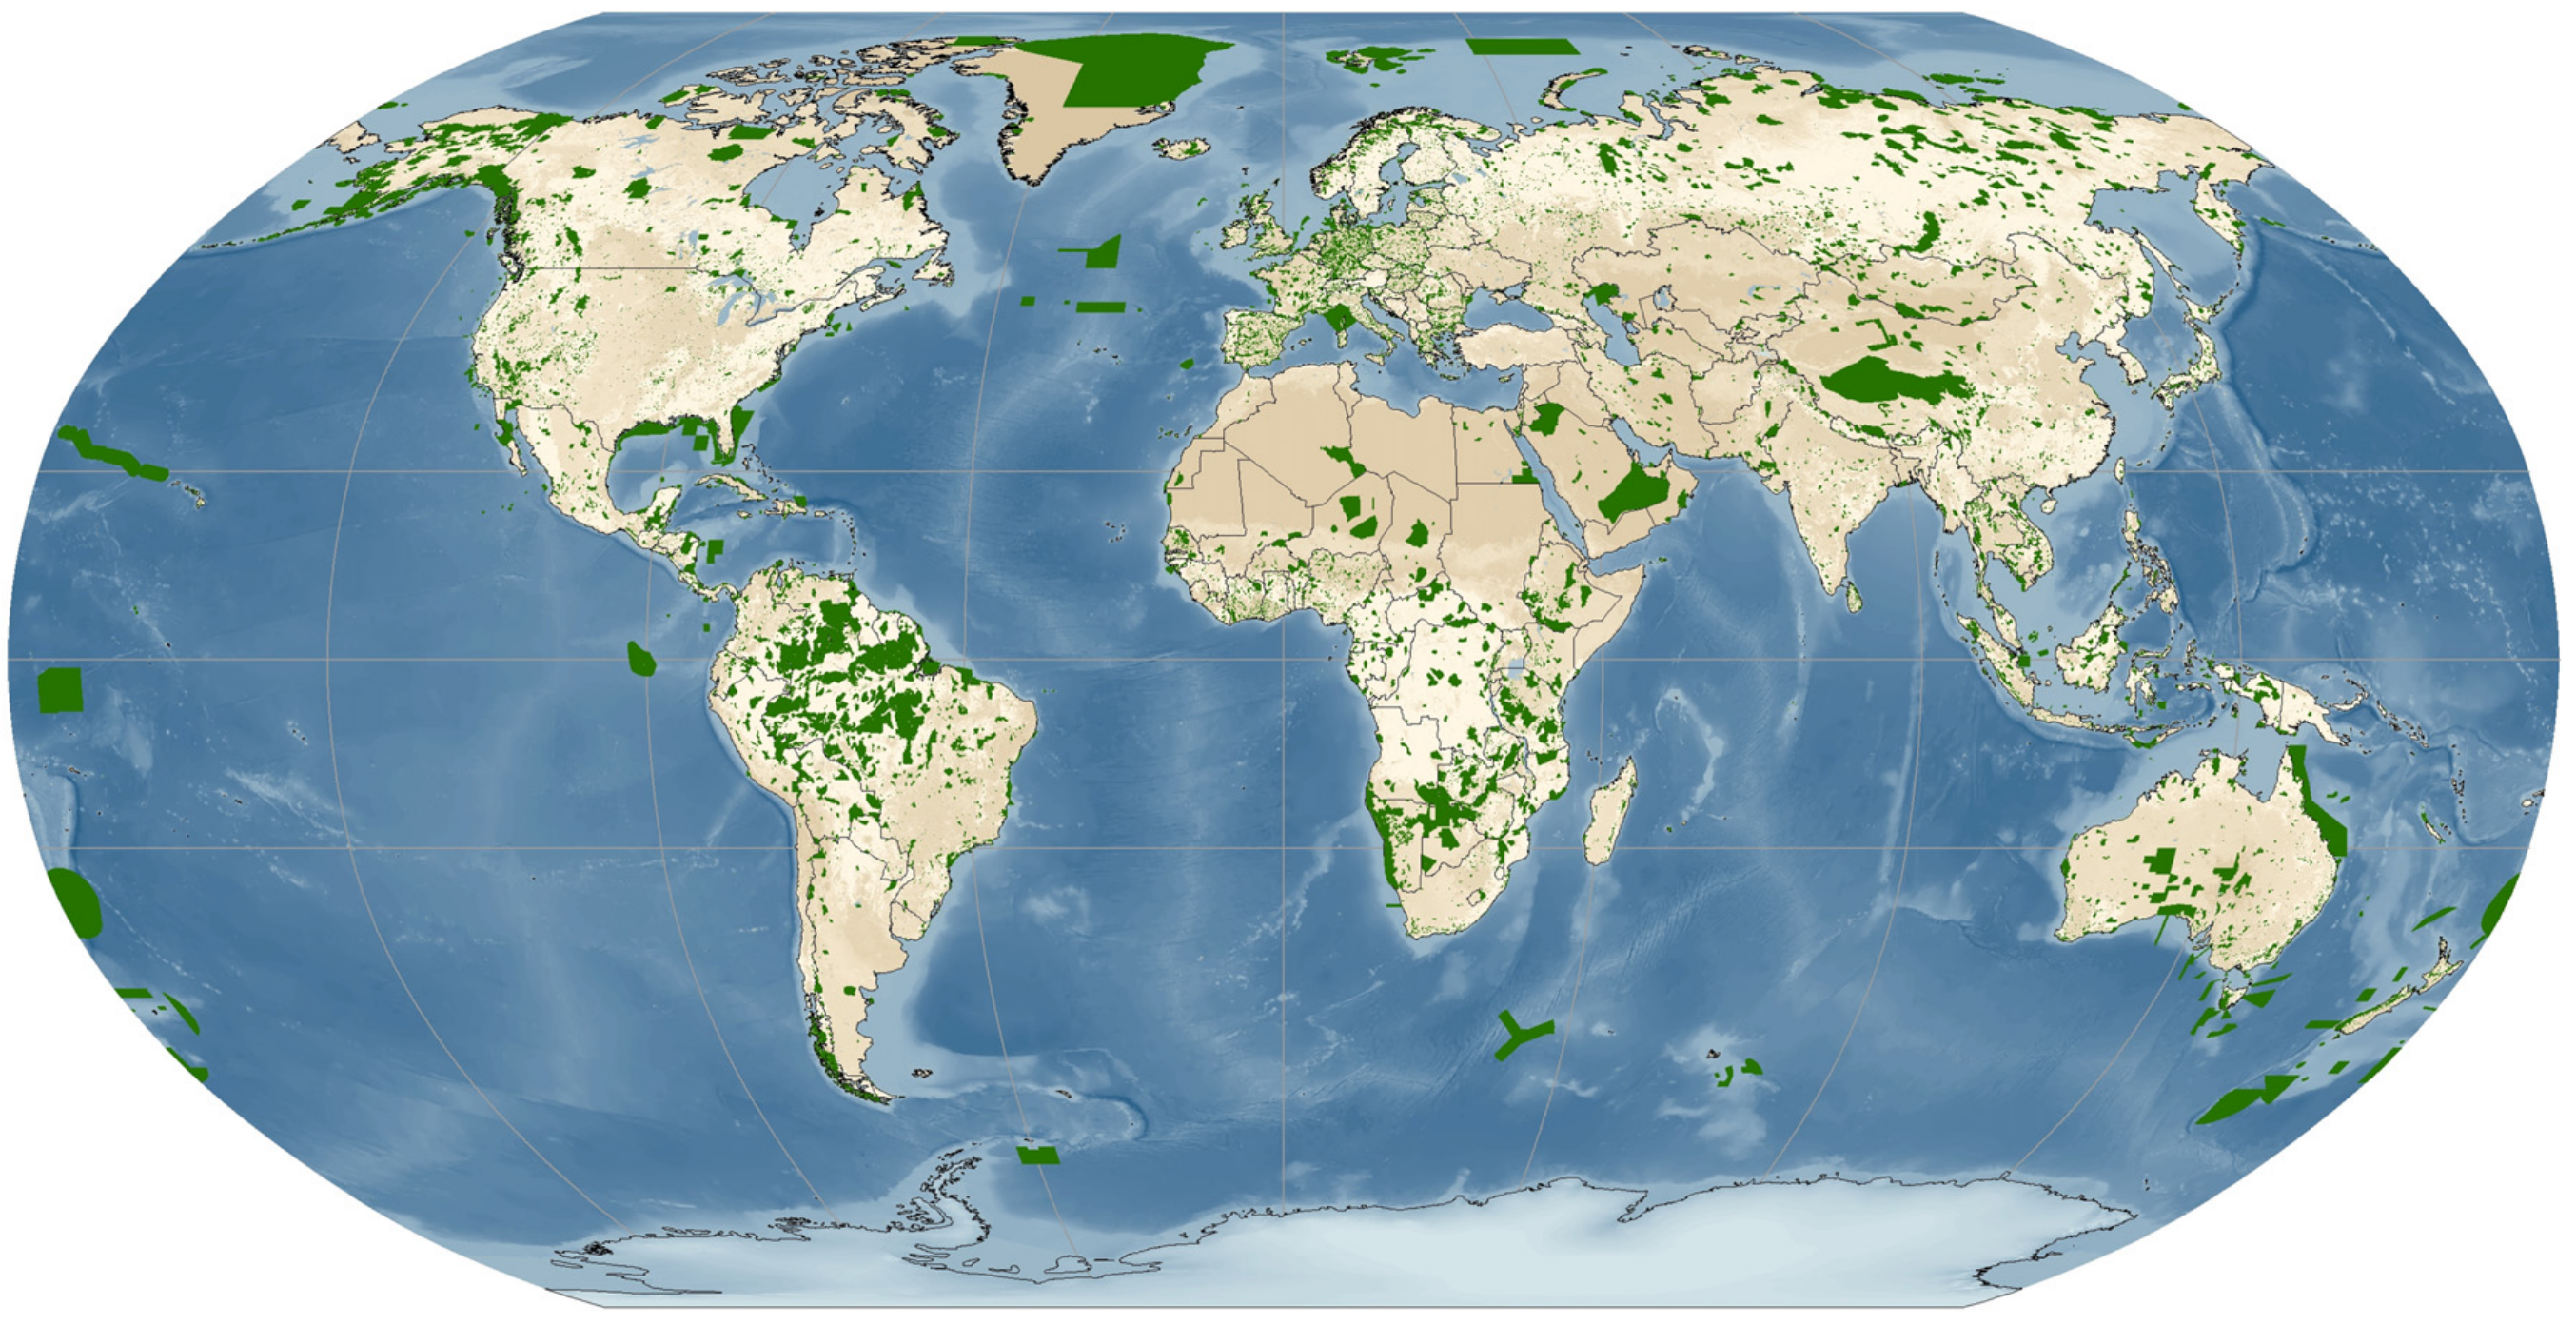
\includegraphics[width=0.8\linewidth]{./../images/global_protected_area_map} \caption{Protected areas of the world. Reproduced from World Database on Protected Areas (WDPA), UNEP-WCMC, July 2011.}\label{fig:global-map}
\end{figure}

\end{frame}

\begin{frame}{Protected area coverage of the world's biomes}
\protect\hypertarget{protected-area-coverage-of-the-worlds-biomes}{}

\begin{table}[t]

\caption{\label{tab:unnamed-chunk-1}Protected area coverage of worlds biomes (in percentage)}
\centering
\fontsize{6}{8}\selectfont
\begin{tabular}{lr}
\toprule
Biome & Percentage cover\\
\midrule
Tropical and subtropical moist broadleaf forests (TMF) & 5.5\\
Tropical and subtropical dry broadleaf forests (TDF) & 5.0\\
Tropical and subtropical coniferous forests (TCF) & 2.5\\
Temperate broadleaf and mixed forests (TeBF) & 3.8\\
Temperatre coniferous forests (TeCF) & 8.8\\
\addlinespace
Boreal forests/taiga (BF) & 6.2\\
Tropical and subtropical grasslands, savannas, and shrublands (TG) & 5.8\\
Temperate grasslands, savannas, and shrublands (TeG) & 2.0\\
Flooded grasslands and savannas (FG) & 8.8\\
Montane grasslands and shrublands (MG) & 3.8\\
\addlinespace
Tundra (T) & 13.8\\
Mediteranean forests, woodlands, and scrub or Sclerophyll forests (MF) & 3.0\\
Deserts and xeric shrublands (D) & 3.8\\
Mangrove (M) & 8.5\\
\bottomrule
\end{tabular}
\end{table}

\end{frame}

\begin{frame}{Protected areas nepal}
\protect\hypertarget{protected-areas-nepal}{}

\begin{table}[t]

\caption{\label{tab:protected-areas-np1}Protected areas of Nepal}
\centering
\fontsize{6}{8}\selectfont
\begin{tabular}{>{\raggedright\arraybackslash}p{8em}>{\raggedright\arraybackslash}p{5em}>{\raggedright\arraybackslash}p{5em}>{\raggedright\arraybackslash}p{6em}>{\raggedright\arraybackslash}p{40em}}
\toprule
S.N Protected Area & Year Established & Area (sq. km.) & Elevation (m) & Conservation Significance\\
\midrule
\rowcolor{gray!6}  1 Chitwan (World Heritage Site 1984) & 1973 & 932 & 150-815 & The Park houses over 50 species of mammals including one-horned rhinoceros, Royal Bengal tiger and bison; Important Bird Area; 539 species of birds that include migrant birds like paradise flycatcher, Indian pitta, parakeets and several species of waterfowl; and many species of amphibians and reptiles including the endangered gharial, marsh mugger crocodile and python. The habitat comprises of deciduous broadleaf forest with over 600 plant species, savannas and wetlands.\\
2 Langtang & 1976 & 1710 & 792-7,245 & The habitat types range from sub-tropical forests below 1,000 m to alpine shrubs and grasslands. Musk deer and red panda are at the focus of conservation. Many other mammals such as snow leopard, wild dog, Himalayan black bear, Himalayan tahr, ghoral, serow, rhesus monkey and langur monkey, and over 370 species of birds including tragopan and impeyan pheasant (danphe) are found.\\
\rowcolor{gray!6}  3 Rara & 1976 & 106 & 1,800-4,048 & Rara has many animal species including endangered red panda and musk deer. Three species of snow trout are found in the lake. During winter over 270 species of birds including coots, great-crested grebe, black-necked grebe, red crested pochard, mallard, common teal, merganser and gulls, and migrant water fowls can be seen. Coniferous forests, primarily of blue pine forms the dominant vegetation. Rhododendron, juniper, spruce, oak and cypress are found around 3,000 m while spruce and fir are more common at higher elevations.\\
4 Sagarmatha (World Heritage Site 1979) & 1976 & 1148 & 2,800-8,848 & The Park is famous for the scenic beauty of the Himalayas (including Mount Everest), musk deer, red panda, beer and snow leopard. Nearly 200 species of birds including impeyan pheasant, blood pheasant, red-billed chough, yellow-billed chough, snow cock, and snow pigeon are found. The forest vegetation comprises of pine and hemlock forests at lower elevations, and silver fir, birch, rhododendron and juniper at higher elevations (i.e. above 3,500 m).\\
\rowcolor{gray!6}  5 Shey-Phoksundo & 1984 & 3555 & 2,000-6,885 & Wild goat (ghoral), blue sheep, musk deer, and the Shey-Phoksundo lake are some of the main attractions. Over 200 species of birds including yellow throated marten, Tibetan partridge, wood snipe, white-throated tit, wood accentor and crimson-eared rose finch, impeyan pheasant, cheer pheasant, chough, raven, Tibetan snow cock, Tibetan twit and Himalayan griffon; and 29 species of butterflies are found. Pine, walnut, willow, oak, cypress are dominant trees in the lower elevations and pine, spruce, juniper and birch at higher elevations. Alpine range is comprised of meadows and shrubs of berberis, wild rose and caragana.\\
\bottomrule
\end{tabular}
\end{table}

\end{frame}

\begin{frame}{}
\protect\hypertarget{section-3}{}

\begin{table}[t]

\caption{\label{tab:protected-areas-np2}Protected areas of Nepal (...continued)}
\centering
\fontsize{6}{8}\selectfont
\begin{tabular}{>{\raggedright\arraybackslash}p{8em}>{\raggedright\arraybackslash}p{5em}>{\raggedright\arraybackslash}p{5em}>{\raggedright\arraybackslash}p{6em}>{\raggedright\arraybackslash}p{40em}}
\toprule
S.N Protected Area & Year Established & Area (sq. km.) & Elevation (m) & Conservation Significance\\
\midrule
\rowcolor{gray!6}  6 Khaptad & 1984 & 225 & 1,000-3,276 & The Park is famous for medicinal plants. Over 220 species of medicinal plants are recorded. Wildlife includes barking deer, wild boar, ghoral, Himalayan black bear, yellow-throated marten, rhesus monkey and langur monkey, and around 270 species of birds are found. Vegetation is mainly comprised of grasslands and subtropical, temperate, and sub alpine forests. This is also a famous spiritual site\\
7 Bardia & 1988 & 968 & 152-1,494 & Mammals such as Royal Bengal tiger, one-horned rhinoceros, elephant, swamp deer, black buck, and reptiles such as gharial, marsh mugger crocodile are the main species. Fresh-water Gangetic dolphin is found in the Karnali River. Bengal florican, lesser florican, silver-eared mesia and sarus crane are some of 400 species of birds found in the Park that is dominated by sal forest and savannahs.\\
\rowcolor{gray!6}  8 Makalu Barun & 1991 & 1500 & 435-8,463 & The park is an important habitat for endangered red panda and snow leopard, and several species of endangered plants. Above 80 varieties of fish including salmon are reported in the Arun River. Wren babbler and olive ground warbler are some of the 400 species of birds found in the Park. Forest vegetation ranges from sub-tropical forests to sub-alpine and alpine vegetation as the elevation increases. The park is also famous for Rhododendrons and orchids.Twenty-five (out of 30 found in Nepal) varieties of rhododendrons, 48 species of orchids, 87 species of medicinal herbs, 48 species o primroses and 86 species of fodder trees are reportedly found in the Park.\\
9 Shivapuri-Nagarjun & 2002 & 159 & 1,366-2,732 & Conservation of watershed that drains the Kathmandu Valley is a major objective. Around 19 species of mammals including Himalayan black bear, leopard, barking deer, wild boar, wild cat, rhesus monkey and langur monkey, 177 species of birds, 102 species of butterflies, and 129 varieties of mushrooms are reported.\\
\rowcolor{gray!6}  10 Banke & 2010 & 550 & 360-480 & Conservation of endangered wildlife and strengthening of transboundary biological corridor are some of the main objectives. Includes eight natural ecosystems, and houses 124 species of plants, 34 mammals, more than 300 birds, 24 reptiles, seven amphibians, and 58 fish species\\
\bottomrule
\end{tabular}
\end{table}

\end{frame}

\begin{frame}{}
\protect\hypertarget{section-4}{}

\begin{table}[t]

\caption{\label{tab:protected-areas-np3}Protected areas of Nepal (...continued)}
\centering
\fontsize{6}{8}\selectfont
\begin{tabular}{>{\raggedright\arraybackslash}p{8em}>{\raggedright\arraybackslash}p{5em}>{\raggedright\arraybackslash}p{5em}>{\raggedright\arraybackslash}p{6em}>{\raggedright\arraybackslash}p{40em}}
\toprule
S.N Protected Area & Year Established & Area (sq. km.) & Elevation (m) & Conservation Significance\\
\midrule
\rowcolor{gray!6}  1 Shuklaphanta & 1976 & 305 & 90-270 & Major wildlife consists of swamp deer, wild elephant, tiger, several species of deer, wild boar, leopard, and monkeys. Marsh mugger crocodile, cobra, and python are Common reptiles.Important Bird Area; Saruscrane,swampfrancolin,grassowl, warblers, flycatchers, Bengal florican are the common birds found in the sub-tropical sal forest and open grasslands.\\
2 Koshi Tappu (Ramsar Site, 1987) & 1976 & 175 & 80-100 & Wild buffalo and Siberian migratory birds are the main focus of conservation. Vegetation consists of grasslands with patches of scrub and deciduous riverine forests. Many other species of mammals (such as wild elephants, wild boar, hog deer, spotted deer, blue bull and jackal); Important Bird Area; 479 species of birds, and reptiles are found. Gangetic dolphins are found in the Koshi River.\\
\rowcolor{gray!6}  3 Parsa & 1984 & 499 & 150-815 & Wildlife species including wild elephant, tiger leopard, sloth bear, and gaur; reptiles including king cobra, common cobra, krait, rat snake and python; over 370 species of birds including the endangered great hornbill are reported. Natural vegetation consists of tropical and sub-tropical sal forests. Chir pine, khair, and sissoo trees are found on the hilly parts.\\
1 Dhorpatan & 1987 & 1325 & 2,850-7,000 & The reserve is famous for blue sheep, which is open for regulated trophy hunting\\
\rowcolor{gray!6}  1 Annapurna & 1992 & 7629 & 1,000-8,092 & Endemic plants and mountains are the main characteristics. Over 100 species of mammals including blue sheep and endangered snow leopard; 39 species of reptiles; 22 species of amphibians; Important Bird Area (IBA); 474 species of birds including multi-colored impeyan pheasant, kokla and blood pheasant are reported. Many species of orchids and rhododendrons are found.\\
\bottomrule
\end{tabular}
\end{table}

\end{frame}

\begin{frame}{}
\protect\hypertarget{section-5}{}

\begin{table}[t]

\caption{\label{tab:protected-areas-np4}Protected areas of Nepal}
\centering
\fontsize{6}{8}\selectfont
\begin{tabular}{>{\raggedright\arraybackslash}p{8em}>{\raggedright\arraybackslash}p{5em}>{\raggedright\arraybackslash}p{5em}>{\raggedright\arraybackslash}p{6em}>{\raggedright\arraybackslash}p{40em}}
\toprule
S.N Protected Area & Year Established & Area (sq. km.) & Elevation (m) & Conservation Significance\\
\midrule
\rowcolor{gray!6}  2 Kanchanjunga & 1997 & 2035 & 1,200-8,598 & Mammals including endangered snow leopard, Himalayan black bear, musk deer, red panda, blue sheep, rhesus monkey; 252 species of different birds including impeyan pheasant, red-billed blue magpie, ashy drongo; 20 indigenous gymnosperms, 15 among Nepal's 23 endemic flowering plants, 30 varieties of rhododendrons and 48 varieties of orchids are reported.\\
3 Manasula & 1998 & 1663 & 1,360-8,163 & Snow leopard, musk deer and Himalayan Tahr are among the 33 species of mammals found in the conservation area. Over 110 species of birds and 1,500-2,000 species of flowering plants are reported.\\
\rowcolor{gray!6}  5 Khairapur & 2010 & 16 & 120-230 & The first organized effort to conserve the endangered blackbuck (Antilope cervicapra).\\
6 Api Nampa & 2010 & 1903 & 539-7,132 & Snow leopard, musk deer, clouded leopard, ghoral, Himalayan black bear and Himalayan tahr are found in the area.\\
\bottomrule
\end{tabular}
\end{table}

\end{frame}

\begin{frame}{Framework for reviewing contribution}
\protect\hypertarget{framework-for-reviewing-contribution}{}

\begin{figure}
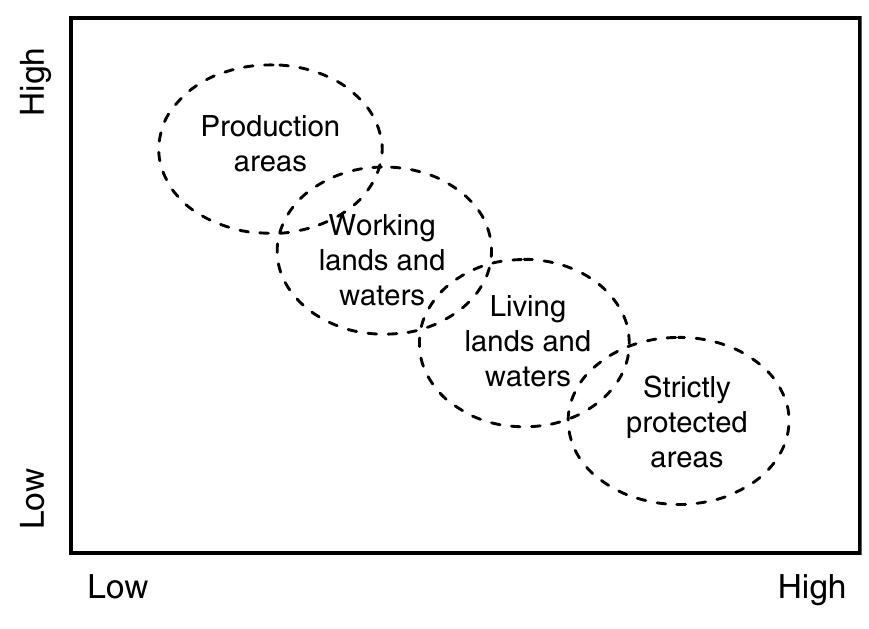
\includegraphics[width=0.45\linewidth]{./../images/contribution_review} \caption{A framework for reviewing the contribution of areas of land and water to biodiversity conservation. Starting at the bottom right hand corner the framework moves from 'strictly protected areas', reflecting the more traditional approach to protected areas managed almost exclusively for biodiversity conservation, The next category is 'living lands and waters', which are areas managed primarily for biodiversity conservation with some extractive uses limited to the ecologically sustainable management of areas of land and water to support life of all forms. 'Working lands and waters' are mostly agricultural lands managed primarily for extractive uses while attempting to conserve biodiversity at the same time. The final category is 'production areas' of land and water where the management focuses exclusively on maximizing extractive and productive uses and biodiversity conservation is not an objective.}\label{fig:contribution-review}
\end{figure}

\end{frame}

\hypertarget{methods-of-biodiversity-conservation}{%
\section{Methods of biodiversity
conservation}\label{methods-of-biodiversity-conservation}}

\begin{frame}{}
\protect\hypertarget{section-6}{}

\begin{enumerate}
\tightlist
\item
  \emph{In situ} conservation;
\item
  \emph{Ex situ} conservation
\item
  Restoration
\end{enumerate}

\end{frame}

\hypertarget{area-specificlocal-approach}{%
\section{Area-specific/local
approach}\label{area-specificlocal-approach}}

\begin{frame}{Farmer as pivot}
\protect\hypertarget{farmer-as-pivot}{}

\begin{itemize}
\tightlist
\item
  Which crop I can cultivate ?
\item
  Which varieties perform good on my locality ?
\item
  Which variety yields better ?
\item
  Which variety can escape disease well ?
\item
  Which crop or crop mixtures are likely to perform well in which season
  ?
\item
  What seed do I store for the upcoming crop ?
\item
  How do I best manage my land to have a good harvest ?
\item
  How do I best preserve the seed to ensure good planting ?
\item
  How do mix or relay my collection of crops where I grow ?
\item
  How do I preserve the integrity of a good variety ?
\end{itemize}

\end{frame}

\begin{frame}{Institutional conservation approaches}
\protect\hypertarget{institutional-conservation-approaches}{}

\begin{itemize}
\tightlist
\item
  Single species based conservation. For e.g. \emph{Ex situ}
  conservation for single species (e.g., zoos, expensive reintroduction
  programs, captive breeding programs).
\item
  Umbrella species approach
\item
  Elimination of invasise species linked to conservation failures.
\item
  Protected areas management, for human exclusion.
\item
  Fragmentation and loss of ecosystem management through management of
  spatial distribution of ecosystem or habitats.
\item
  Incorporation of short-frequency disturbances.
\item
  Limitting or excluding human extraction of resources from nature
  reserves.
\item
  Reserve design and size allocation based on territory need of each
  species.
\item
  Use of corridors and buffer zones to link habitat fragments and
  reserve networks.
\item
  Small-scale, data-intensive species and community model design and
  implementation.
\item
  Development of nonmarket values for species.
\end{itemize}

\end{frame}

\hypertarget{national-nepalsregional-approaches}{%
\section{National (Nepal's)/regional
approaches}\label{national-nepalsregional-approaches}}

\begin{frame}{Targeted approach}
\protect\hypertarget{targeted-approach}{}

\begin{enumerate}
\tightlist
\item
  Management of protected areas
\end{enumerate}

\begin{itemize}
\tightlist
\item
  A: Improvement in management of protected areas and species.
\item
  B: Abatement in poaching and illegal trade of wildlife and wildlife
  parts
\item
  C: Improvement in protected area habitats and connectivity
\item
  D: Improvement in management of protected area tourism
\end{itemize}

\begin{enumerate}
\setcounter{enumi}{1}
\tightlist
\item
  Management of biodiversity outside protected area
\end{enumerate}

\begin{itemize}
\tightlist
\item
  A: Improvement in forest governance and management
\item
  B: Significant reduction (by at least 75\% of the current rate) in the
  loss and degradation of forest
\item
  C: Improvement in conservation of biodiversity in community managed
  forests
\item
  D: Enhancing conservation of species and genetic diversity
\item
  F: Enhancing forest based livelihoods
\end{itemize}

\end{frame}

\begin{frame}{Targeted approach (\ldots{}continued)}
\protect\hypertarget{targeted-approach-continued}{}

\begin{enumerate}
\setcounter{enumi}{2}
\tightlist
\item
  Management of rangeland biodiversity
\item
  Management of watershed biodiversity
\item
  Management of agrobiodiversity
\item
  Management of mountain biodiversity
\end{enumerate}

\end{frame}

\begin{frame}{Cross-thematic and cross-sectoral strategies}
\protect\hypertarget{cross-thematic-and-cross-sectoral-strategies}{}

\begin{itemize}
\tightlist
\item
  Addressing the policy and legislative gaps
\item
  Institutional strengthening
\item
  Mainstreaming biodiversity across the government, society and economy
\item
  Harmonization of biodiversity related international conventions
\item
  Enhancement of national capacity for improved management of
  biodiversity
\item
  Landscape management
\item
  Management of invasive alien species
\item
  Adaptation to and mitigation of the effects of climate change
\item
  Integrating gender and social inclusion perspectives
\item
  Conservation of and Respect to Traditional Knowledge, Innovations and
  Practices of Indigenous and Local Communities
\item
  Knowledge generation and management
\item
  Technology development, acquisition and use
\item
  Communication, extension and outreach
\item
  Fund generation and mobilization
\item
  Monitoring evaluation and reporting
\end{itemize}

\end{frame}

\begin{frame}{Cross sector}
\protect\hypertarget{cross-sector}{}

\end{frame}

\begin{frame}{Sectoral}
\protect\hypertarget{sectoral}{}

\end{frame}

\hypertarget{international-convention-and-treaties}{%
\section{International convention and
treaties}\label{international-convention-and-treaties}}

\hypertarget{intellectual-property-rights}{%
\section{Intellectual property
rights}\label{intellectual-property-rights}}

\hypertarget{bibliography}{%
\section{Bibliography}\label{bibliography}}

\end{document}
